\documentclass[thesis-solanki.tex]{subfiles}


\ifMain
\externaldocument{thesis-solanki}
\fi
\begin{document}

\chapter{Prototype 2.1}{\label{proto2.1}}

\section{About this chapter}
This chapter attempts to infuse the generic methodology from \ref{proto1} in a current \progLang{Prolog} implementation \cite{prolog-lib}
and make the unification ``monadic''.

\section{How prolog-0.2.0.1 works}

As described in the previous chapter about extending languages to incorporate functionality, this prototype applies the procedure to the
eDSL in \cite{prolog-lib}.

The original abstract syntax used by the library,
\begin{code-list}[h]
\begin{minted}[linenos]{haskell}

data VariableName = VariableName Int String
      deriving (Eq, Data, Typeable, Ord)

type Atom         = String

data Term = Struct Atom [Term]
          | Var VariableName
          | Wildcard -- Don't cares
          | Cut Int
      deriving (Eq, Data, Typeable)

data Clause = Clause { lhs :: Term, rhs_ :: [Goal] }
            | ClauseFn { lhs :: Term, fn :: [Term] -> [Goal] }
      deriving (Data, Typeable)

type Goal         = Term
type Program      = [Clause]
\end{minted}
\caption{Current Language Implementation}
\label{tab:currlangimpl}
\end{code-list}

From the Figure~\ref{tab:currlangimpl} we will focus on the \textit{Term} since the others just add wrappers around expressions which can
be created by it. The above language suffers from most of the problems discussed in the previous chapter. The above is used to construct
\progLang{Prolog} ``terms'' which are of a ``single type''.


The implementation consists of components that one would find in a Language Processing System \ref{fig:A language-processing system},

\begin{figure}[th]
\centering
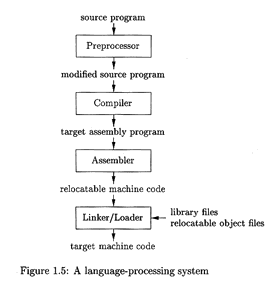
\includegraphics[scale = 0.7]{Language_Processing_System.png}
\caption{A language-processing system \cite{Aho:1986:CPT:6448}}
\label{fig:A language-processing system}
\end{figure}

specifically speaking, parts of a compiler \ref{fig:Phases of Compiler},

\begin{figure}[th]
\centering
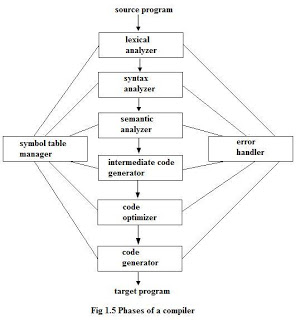
\includegraphics[scale = 0.7]{Phases_of_compiler.jpg}
\caption{Phases of Compiler \cite{Aho:1986:CPT:6448}}
\label{fig:Phases of Compiler}
\end{figure}

The architecture for a compiler as described in \ref{fig:Phases of Compiler} would not be needed since \progLang{Haskell} provides most of
them. Nonetheless, the library has the following major components,

\begin{enumerate}
\item Syntax, defining the language.

\item Database, to create a storage for the expressions.

\item Parser.

\item Interpreter.

\item Unifier.

\item Read-Eval-Print Loop(REPL). 
\end{enumerate}

To prove the modularity of the approach for language modification and monadic unification only the abstract syntax and unifier will be
customized.


\clearpage
\section{What we do in this prototype?}
In the first prototype we just did unification of two terms not query resolution.

We do complete \progLang{Prolog} query resolution like stuff.

\ref{proto1} provides a generic procedure / methodology to convert a language into monadic unifiable form

\clearpage
\section{Current implementation (prolog-0.2.0.1)}

Beginning with language from Figure~\ref{tab:currlangimpl} is transformed into an isomorphically equivalent grammar described in 
Figure~\ref{tab:flatgrp0201}

\begin{code-list}[h]
  \begin{singlespace}
    \inputminted[linenos]{haskell}{haskell-proto2-flattened-rarefy.hs}
  \end{singlespace}
  \caption{Flattened (non-recursive) grammar}
\label{tab:flatgrp0201}
\end{code-list}

\clearpage

The current unification uses basic pattern matching to unify the terms. 

The process returns a Unifier,
\begin{code-list}[h]
\begin{minted}[linenos]{haskell}
type Unifier      = [Substitution]
type Substitution = (VariableName, Term)
\end{minted}
\caption{prolog-0.2.0.1 Unifier}
\label{tab:prlg0201unifier}
\end{code-list}



Figure~\ref{tab:prlg0201unifier} shows the result type. The instances are created to open up the language and make it compatible with the
unification library \cite{prolog-lib}.

\clearpage

Coming back to the unification itself shown in Figure~\ref{tab:prlg0201unification}. Each language expression is matched based on its 
structure.
  
\begin{code-list}[h]
  \begin{singlespace}
    \inputminted[linenos]{haskell}{haskell-proto2-unification-lion.hs}
  \end{singlespace}
\caption{prolog-0.2.0.1 Unification}
\label{tab:prlg0201unification}
\end{code-list}

The issue with the current appraoch is the rigidity of the procedure. Any language modification will cause a ripple effect across the 
system. As described in Chapter~\ref{proto1}, the advantages of \textit{functorizing} language hold in this implementation as well.

\clearpage
\section{Modifications}
The resulting language is not far from what we did in \ref{proto1} apart from the fact that the \textit{Term} expressions are encapsulated
to form \textit{Clauses} which in turn form a \textit{Program}.

Moreover, the required instances make the language compatible with the unification procedure.

\begin{singlespace}
  \inputminted[linenos]{haskell}{haskell-proto2-starry-forked.hs}
\end{singlespace}

Aditionally helper functions for converting expressions between the two domains and translation to \textit{UTerm}.

To solve the issue of infinitely deep language expressions, we find the fixed point of the expression. The unification function provided by 
\cite{prolog-lib} is not very \progLang{Prolog} like\eref{language-like} in nature and certain adjustments need to be made. 
\begin{enumerate}
\item Extracting variable and creating dictionaries.

\item Converting to UTerms and back
\end{enumerate}

\begin{singlespace}
  \inputminted[linenos]{haskell}{haskell-proto2-clean-lemur.hs}
\end{singlespace}

Take original expressions flatten fix convert unify
run it STBinding monad to extract substitutions.

\begin{singlespace}
  \inputminted[linenos]{haskell}{haskell-proto2-hearty-kayo.hs}
\end{singlespace}



\section{Results}

It works,



\section{Chapter Recapitulation}

\ifMain
\begin{scope}
  \nolinenumbers
  \enotesize
  \par
  \begin{singlespace}
  \setlength{\parskip}{12pt plus 2pt minus 1pt}
  \theendnotes
  \par
  \end{singlespace}
\end{scope}
\unbcbibliography{bibliography}
\fi

\end{document}
